% The draft script for CGI 2022
% Version: 1.0
% Due date (Abstract): N.A.
% Due date (Full Paper): Mar. 10, 2022
% Pages: 8-12

\RequirePackage{fix-cm}
% \documentclass{svjour3}
% \documentclass[smallcondensed]{svjour3}
% \documentclass[smallextended]{svjour3}
% \documentclass[twocolumn,draft]{svjour3}
\documentclass[twocolumn]{svjour3}
\smartqed  % flush right qed marks

% ========================= PACKAGES ============================
\usepackage{graphicx}
\usepackage{cite}
\usepackage{amssymb}
\usepackage{booktabs}
\usepackage{xspace}
\makeatletter
\DeclareRobustCommand\onedot{\futurelet\@let@token\@onedot}
\def\@onedot{\ifx\@let@token.\else.\null\fi\xspace}
\def\eg{\emph{e.g}\onedot} \def\Eg{\emph{E.g}\onedot}
\def\ie{\emph{i.e}\onedot} \def\Ie{\emph{I.e}\onedot}
\def\cf{\emph{c.f}\onedot} \def\Cf{\emph{C.f}\onedot}
\def\etc{\emph{etc}\onedot} \def\vs{\emph{vs}\onedot}
\def\wrt{w.r.t\onedot} \def\do   25f{d.o.f\onedot}
\def\etal{\emph{et al}\onedot}
\makeatother
\usepackage{xcolor}
\usepackage{multirow}
\usepackage{threeparttable}
\graphicspath{{assets/}}                              % set paths
\DeclareGraphicsExtensions{.pdf,.jpeg,.png}      % set extensions

\journalname{CGI2022}                     % Entered by the editor
\begin{document}

% ====================== TITLE & AUTHORS ========================
\title{Engagement Estimation of the Elderly from Wild Multiparty Human-Robot Interaction}
\subtitle{}
\author{Anonymous Submission}
%\author{Zhijie~Zhang \and Jianmin~Zheng \and Gauri~Tulsulkar \and Nidhi~Mishra \and Nadia~Magnenat~Thalmann}
\institute{Address(es) of author(s) should be given here.}
%\institute{
%%Z. Zhang \and J. Zheng
%%\at School of Computer Science and Engineering, Nanyang Technological University, Singapore.\\
%%\email{\{zhijie002, asjmzheng\}@ntu.edu.sg}
%%\and
%%G. Tulsulkar \and N. Mishra
%%\at Institute of Media Innovation, Nanyang Technological University, Singapore.
%%\and
%%N. M. Thalmann
%%\at MIRALab, University of Geneva, Switzerland.\\
%%\email{thalmann@miralab.ch}
%%}
\date{}                                   % Entered by the editor
\maketitle

% ==================== ABSTRACT & KEYWORDS ======================
\begin{abstract}
The use of social robots in clinical treatment or nursing homes to assist the elderly and their caregivers will be becoming common, where robots' understanding of engagement of the elderly is important. Traditional engagement estimation often requires expert involvement and is in controlled dyadic interaction environment. In this paper, we propose a supervised machine learning model to estimate the engagement state of the elderly in a multiparty human-robot interaction (HRI) scennario from the real-world video recording as input. The model is built upon the basic concept of engagement in geriatric psychiatry and HRI video representations. It adapted pre-trained models to extract behavior, affective and visual signals as the multi-modal features to estimate the engagement. The model is formed by a self-attention mechanism for individual learning and a graph attention neural network for group learning.  
We test the proposed method using 43 wild multiparty elderly-robot interaction videos.  The results show that our model is capable of detecting the key participants and estimating the engagement of the elderly. Moreover, information from the surroundings can considerably improve the estimation results.
\keywords{human-robot interaction \and engagement estimation \and affective computing \and multiparty}
\end{abstract}

% ======================= INTRODUCTION ==========================
\section{Introduction}
\label{s:Introduction}

This paper considers the problem of estimating the engagement of the elderly in wild multiparty human-robot interaction (HRI). With the advance of social robots, deploying robots in the healthcare becomes a possible solution to providing round-the-clock medical and psychological care to the elderly, especially the people with dementia (PwD), and supporting their caregivers as well~\cite{Ghafurian2021Social, Perugia2020ENGAGEDEM}. Natural elderly-robot interaction helps make the robot a good companion for the elderly who usually experience declines in physical and cognitive capacities. This has great impact since the proportion of people aged 60 years and older in the world will nearly double from 12\% in 2015 to 22\% in 2050 according to the World Health Organization~\cite{WHO2021Ageing}. 

During the elderly-robot interaction, if the robot can recognize the engagement state of the elderly, this helps the robot to respond to the elderly properly to maintain long-term interaction or to produce appropriate social behavior for the elderly to feel a sense of belonging. Here engagement refers to the inner state of a participant attributing to being together with the other participants and continuing the interaction~\cite{Poggi2013Mind}. Many studies have shown that the engagement plays an important role in both human-human interaction (HHI) and human-robot interaction~\cite{Jones2018Engagement}. 

\begin{figure}[t]
  \centering
  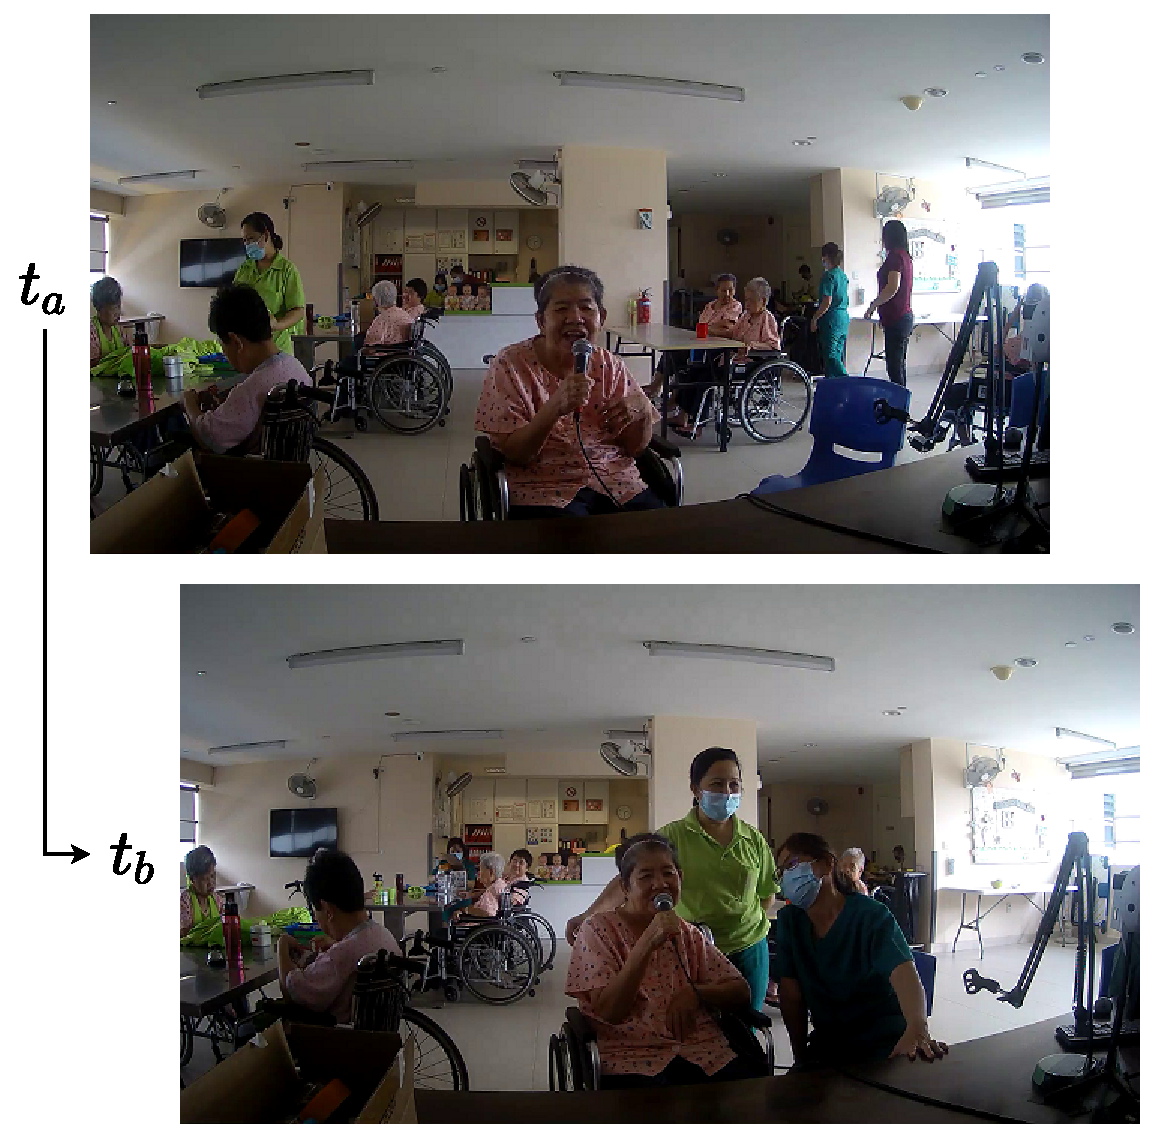
\includegraphics[width=\linewidth]{assets/interaction_sample.drawio.pdf}
  \caption{Two sample frames from a video recording of real-world multiparty HRI demonstrate conversation dynamics (from one to three participants) and unconstrained environment (open space and free-moving background people). The video is recorded from robot ego-view, and $t_a, t_b$ denote two time stamps.}
  \label{f:interaction_sample}
\end{figure}

Engagement estimation is kind of affective computing and behavior recognition, and it goes further to probe the inner intention behind the apparent behavior and emotion. Many methods have been developed to estimate engagement in various scenarios such as general HRI~\cite{Salam2017Fully, Celiktutan2019Multimodal, BenYoussef2019Early, Saleh2021Improving}, museum tour guide~\cite{DelDuchetto2020Are}, classroom or distance learning~\cite{BenEliyahu2018Investigating, Zhu2020Multirate, Rudovic2019Personalized, Sumer2021Multimodal, Monkaresi2017Automated, Abedi2021Affectdriven, Gao2020NGage}, and  healthcare~\cite{Anagnostopoulou2021Engagement, Jain2020Modeling, Jones2018Engagement, Steinert2020Engagement}. Conventional approaches use nonverbal cues such as proxemics, body pose, gaze patterns, facial expressions, and context information to build engagement estimation classifiers. Deep learning approaches are also developed for engagement estimation~\cite{DelDuchetto2020Are,Zhu2020Multirate,Guhan2020ABCNet,Saleh2021Improving,Sumer2021Multimodal,Anagnostopoulou2021Engagement}. However, most previous work assumes that the interaction is in a laboratory environment or a dyadic setting. 
When the research is expanded to special populations and more complex circumstances as this paper is (see Fig.~\ref{f:interaction_sample} for example), not much work has been done before. This may be in part due to the following challenges:
\begin{enumerate}
  \item[C1] The non-verbal signals from \textbf{the elderly} alter in facial shape and patterns of body behaviors along with aging~\cite{Guo2013Facial, Folster2014Facial}. This challenges the conventional computer vision approaches in accurately estimating engagement state.
  \item[C2] From dyadic to \textbf{multiparty HRI}, understanding the dynamics and stability of the interaction becomes more complicated.
  \item[C3] In unconstrained \textbf{wild} space, moving people, bad lighting, confusing objects, etc. make it difficult to interpret the complex environment.
\end{enumerate}

To tackle these challenges, in this paper we propose a supervised learning method for estimating engagement from real-world multiparty elderly-robot interaction. It takes video sequences as input and outputs the estimated engagement state. Fig.~\ref{f:architecture} shows the whole process. For each video clip, we first extract  behavioral, affective, and visual feature maps. We adapt ResNet-3D~\cite{Hara2018Can} as the backbone to generate behavioral features from spacetime region. Affective and visual representations of participants are extracted using emotion recognition and face analysis tool. Then, we feed these features into an individual learning module, where features are refined by a self-attention mechanism. After that, the refined features are fed to the group learning module, which is a graph attention network learning the relationships among participants. The relationship conveys side participants' information, which helps the engagement estimation of the key elderly. Furthermore, to support the supervision, we label a real-world dataset, which is the video recording of the interaction between the elderly and an intelligent social robot, following the conventional psychological approach. The main contributions of the paper are
\begin{itemize}
\item We propose an automated approach to analyze wild multiparty HRI videos and estimate the engagement of the elderly.
\item We borrow the concept of engagement components from psychiatry to design our network investigating behavioral, affective, and visual features.
\item We build a machine learning model consisting of the self-attention network and the graph attention neural network for individual and group learning, which efficiently use both individual and group information to  improve engagement estimation.
\item We create a labeled engagement dataset from a video recording of multiparty elderly-robot interaction in a wild environment.
\end{itemize}


%This paper is organized as follows. Sec.~\ref{s:Related_Work} presents the related work of engagement estimation in HRI, especially for the elderly. Sec.~\ref{s:Engagement_Estimation_of_the_Elderly} describes our proposed approach for estimating the engagement in a real-world scenario and the method of detecting main conversation group members. In Sec.~\ref{s:Experiments_and_Results}, we elaborate the dataset we collected and used for our experiments, as well as the annotation process. The details of the implementation, evaluation metrics, and main results are also presented. Finally, Sec.~\ref{s:Conclusions} summarizes the paper and outlines possible future work.

\begin{figure}[t]
  \centering
  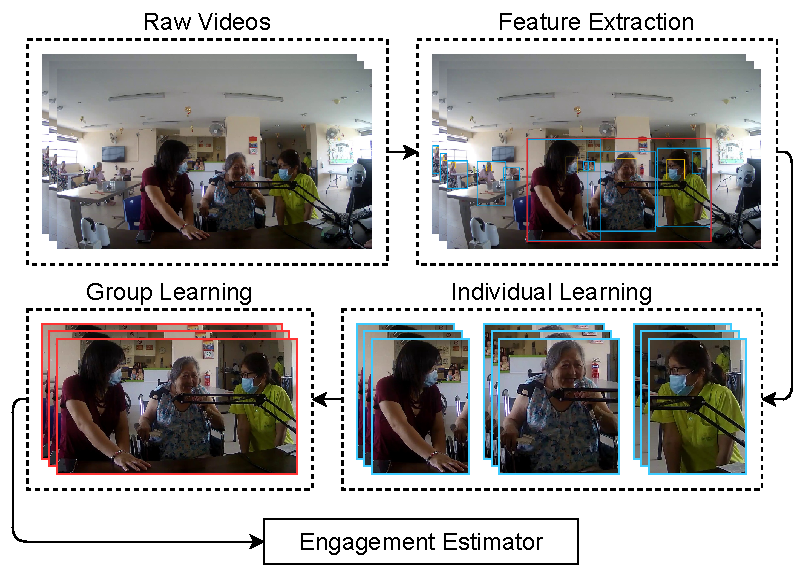
\includegraphics[width=\linewidth]{assets/architecture.drawio}
  \caption{Overview of the proposed engagement estimation. The method is composed of four modules: (i) Feature Extraction, (ii) Individual Learning, (iii) Group Learning, and (iv) Engagement Estimation.}
  \label{f:architecture}
\end{figure}


\begin{table*}[htb!]
  \centering
  \caption{Comparison of Engagement Estimation Methods}
  \label{t:references}
  \begin{threeparttable}[b]
  \begin{tabular}{p{0.06\linewidth}p{0.08\linewidth}p{0.12\linewidth}p{0.11\linewidth}p{0.23\linewidth}p{0.25\linewidth}}
  \toprule
  \textbf{Paper} & \textbf{Scenario} & \textbf{Participants}\tnote{1} & \textbf{Modality(s)}\tnote{2} & \textbf{Approach} \tnote{3} & \textbf{Output}\tnote{4} \\
  \midrule
  \cite{BenYoussef2019Early} & HRI & I/G & vis, aud & LR & $\hat{y} \in$ \{NBrk, Brk\} \\
  \cite{Gao2020NGage} & HHI & G (age 15-17) & phy, env & LightGBM & $\hat{y} \in$ [1, 5] \\
  \cite{Monkaresi2017Automated} & HCI & I (age 20-60) & vis & NB & $\hat{y} \in$ \{Eng, NEng\} \\
  \cite{Salam2017Fully} & HRI & M & vis, dpt, per & SVM \& RF & $\hat{y} \in$ \{Eng, NEng\} \\
  \midrule
  \cite{Anagnostopoulou2021Engagement} & HRI & I/G (children) & vis, dpt & AlexNet \& 2D CNNs & $\hat{y} \in$ \{Eng, MEng, NEng\} \\
  \cite{DelDuchetto2020Are} & HRI & I/G & vis & CNNs+LSTM & $\hat{y} \in$ [0, 1] \\
  \cite{Guhan2020ABCNet} & HHI/HCI & I & vis, aud, txt & GANs & $\hat{y} \in$ \{Eng, NEng\} \\
  \cite{Rudovic2019Personalized} & HRI & I (age 4-6) & vis & RL & $\hat{y} \in$ \{HEng, MEng, LEng\} \\
  \cite{Saleh2021Improving} & HRI & I/G & vis & I3D & $\hat{y} \in$ \{Eng, NEng\} \\
  \cite{Steinert2020Engagement} & HCI & I (PwD) & vis & LSTM & $\hat{y} \in$ \{Eng, MEng, NEng\} \\
  \cite{Sumer2021Multimodal} & HHI & G (students) & vis & MLP \& LSTM & $\hat{y} \in$ \{HEng, MEng, LEng\} \\
  \cite{Zhu2020Multirate} & HCI &
  I (age 19-27) & vis & GRU & $\hat{y} \in$ \{HEng, Eng, BEng, NEng\} \\
  \midrule
  \textbf{Ours} & HRI & M (PwD) & vis & ResNet3D+Attention+GAT & $\hat{y} \in$ [0, 1] \\
  \bottomrule
  \end{tabular}
  \begin{tablenotes}
    \item [1] I, G, and M denote individual, group, and multiparty. The difference between multiparty and group is that multiparty treats participants separately but group treats them as a whole.
    \item [2] Modalities: vis = visual, dpt = depth, per = personality, aud = audio, phy = physiological, env = environmental, and txt = text.
    \item [3] Symbol `\&' indicates using both and comparing with each other, and symbol `+' means combining to form a framework.
    \item [4] $\hat{y}$ represents the inferred engagement label or value. For classification, Eng = Engage, Brk = Breakdown. The letters before Eng and Brk are N = Not, H = Highly, B = Barely, and M = Medium.
  \end{tablenotes}
 \end{threeparttable}
\end{table*}

% ======================= RELATED WORK ==========================
\section{Related Work}
\label{s:Related_Work}
%The estimation of engagement encompasses areas from computer vision to psychological science and psychiatric nursing. 
This section briefly reviews some relevant work, especially in engagement estimation and engagement studies on geriatric psychiatry.

%%%%%%%%%%%%%%%%%%%%%%%%%%%%%%%%%%%%%%%%%%%%%%%
\subsection{Engagement Estimation}
\label{subs:Automated_Engagement_Estimation}

Traditional engagement estimation~\cite{Salam2017Fully, Celiktutan2019Multimodal, BenYoussef2019Early, Monkaresi2017Automated, Gao2020NGage} extracts high-level social features, for example, body pose, facial expressions, gaze and task-related information, followed by a machine learning classifier. These features are intuitive and can be used with unimodal and multimodal combinations.  Recently, with great progress of machine learning in computer vision, more and more deep learning methods have been developed for engagement estimation~\cite{Saleh2021Improving, DelDuchetto2020Are, Zhu2020Multirate, Guhan2020ABCNet, Rudovic2019Personalized, Sumer2021Multimodal, Anagnostopoulou2021Engagement}. A summary of the estimation methods is given in Table~\ref{t:references}, which also includes our proposed method for comparison.

\textbf{Machine Learning Classifiers.} In general HRI, Salam \etal~\cite{Salam2017Fully} classified engagement using support vector machine (SVM) and random forest (RF), depending on predicted personality in a triadic interaction. They advanced the concept of engagement to the group level and claimed that categorization of engagement based on individual and interpersonal features without personality is insufficient. A similar work was proposed in \cite{Celiktutan2019Multimodal}. Ben-Youssef \etal~\cite{BenYoussef2019Early} studied engagement in HRI from the breakdown perspective, \ie, users leave before the expected end. They extracted nonverbal multimodal data such as the distance to the robot, gaze and head motion, facial expressions, and audio. A logistic regression (LR) classifier was used. 

Another widely investigated situation is online or in-class learning. Monkaresi \etal~\cite{Monkaresi2017Automated} explored engagement in the situation where students completed an online writing activity. Heart rate, action units (AUs) and local binary patterns were extracted and fed to a set of classifiers like Naive Bayes (NB). Gao \etal~\cite{Gao2020NGage} predicted high school students' learning engagement including emotional, behavioral, and cognitive engagement in real-world classes. They used a set of features from wearable and indoor weather sensors to infer students' engagement status.

\textbf{Deep Neural Networks.} The aforementioned approaches require expert design of input features and cannot efficiently deal with large feature dimensions. Del Duchetto \etal~\cite{DelDuchetto2020Are} proposed a regression model based on CNNs and Long Short-Term Memory (LSTM) networks, which allows robots to compute the engagement from ego-view HRI videos. The model was built on a long-term dataset from an autonomous tour guide robot in a museum. Zhu \etal~\cite{Zhu2020Multirate} presented an attention-based Gated Recurrent Unit network to predict engagement of students learning online. Taking the advantage of the published dataset~\cite{BenYoussef2019Early}, Saleh \etal~\cite{Saleh2021Improving} applied Inflated 3D ConvNets architecture to predict engagement state in an end-to-end way.

To estimate the engagement of children with autism spectrum disorder interacting with robots, Anagnostopoulou \etal~\cite{Anagnostopoulou2021Engagement} compared AlexNet~\cite{Krizhevsky2012Imagenet} and 2D CNNs using 2D or 3D poses. Rudovic \etal~\cite{Rudovic2019Personalized} proposed  personalized reinforcement learning (RL) to estimate engagement level (low, medium, high) from videos of child-robot interactions. The videos were labeled offline by experts, and used to personalize the policy and engagement classifier to a target child over time.

For HHI, Sumer \etal~\cite{Sumer2021Multimodal} utilized video recordings of classes to get attentional and emotional engagement features, and then applied SVM, RF, multilayer perceptron (MLP), and LSTM to predict students' engagement levels. Guhan \etal~\cite{Guhan2020ABCNet} described a multimodal GAN-based approach, called ABC-Net, to identify engagement from online dyadic HHI recordings. They utilized three-branch networks to gain valence and arousal, from which they generated engagement labels.

%%%%%%%%%%
\subsection{Engagement in Geriatric Psychiatry}
\label{subs:Engagement_for_the_Elderly}

In geriatric psychiatry, the concept and measurement of engagement is well established. For example, Cohen-Mansfield \etal proposed an Observational Method of Engagement for PwD~\cite{Cohen2009Engagement}, which was one of the most well-known tools that many studies have used to measure engagement~\cite{Trahan2014Systematic}. Following this concept, Jones \etal~\cite{Jones2018Engagement} developed the Engagement of a Person with Dementia Scale (EPWDS) towards psychosocial activities by assessing the behavioral and emotional expressions and responses. In~\cite{Perugia2020ENGAGEDEM}, an affective computing framework was presented, which specifies the components of engagement in HRI.

Moreover, robotic and computer assistance has been shown to be an effective intervention. Moyle \etal~\cite{Moyle2017Use} designed a robot seal for PwD. They found that the robot seal was more effective than usual care in improving mood states and agitation and participants were more engaged with it than with a toy. Similarly, Feng \etal~\cite{Feng2021ContextEnhanced} introduced an interactive system involving a display and a robotic sheep to engage PwD. They claimed that multimodal stimuli played a significant role in promoting engagement.

However, all the previously mentioned  methods require expert involvement for engagement estimation. To achieve automated estimation, Steinert \etal~\cite{Steinert2020Engagement} proposed a vanilla LSTM model to predict emotional engagement based on visual facial features (extracted by OpenFace~\cite{Baltrusaitis2018OpenFace} and VGGFace~\cite{Parkhi2015Deep}) and contextual information (daytime, wellbeing, \etc). Similar to \cite{Steinert2020Engagement}, our work is also an automated method. We use not only visual facial features, but also affective features, behavior features and the relation among all participants in the main interaction group.


% ==========================================
%%==========================================
\section{Concept of Engagement}
\label{subs:What_Is_Engagement}
Engagement is generally regarded as a state or a process. According to Oertel \etal~\cite{Oertel2020Engagement}, this notion is ambiguous across different domains. While in terms of the state participants are either engaged or not engaged, by process the concept emphasizes how  interactors establish, maintain, and complete their perceived connection to each other during an interaction~\cite{Sidner2005Explorations}.
Note that the term  {\em state}  represents objectively observed facts in HHI or HRI, which is whether the participants are within interaction or not.
It is used to distinguish itself from \textit{process}. In this paper, we adopt the definition of engagement from~\cite{Poggi2013Mind}, which refers to the participant's inner state of being together with other participants and continuing the interaction.

\subsection{Elements of Engagement} 
In general, engagement contains several elements~\cite{Castellano2009Detecting, Guhan2020ABCNet, Sumer2021Multimodal, Christenson2012Handbook, OBrien2008What, CohenMansfield2011Comprehensive, Archambault2017Joint, BenEliyahu2018Investigating, Corrigan2016Engagement, Perugia2020ENGAGEDEM}. They usually include behavioral, affective, visual, verbal, social, and cognitive signals. 
\begin{itemize}
  \item \textbf{Behavioral} involves observable behaviors such as approaching, touching, avoiding, and hitting.
  \item \textbf{Affective} is defined as the reactions that are usually represented by the valence and arousal.
  \item \textbf{Visual} encompasses actions involving the eyes and head such as maintaining contact or appearing inattention to others or materials.
  \item \textbf{Verbal} reflects the sounds and semantic information towards other participants.
  \item \textbf{Cognitive} refers to psychological investment and effort allocation of the person in order to fully comprehend the situation.
  \item \textbf{Social} includes the activities of encouraging or disrupting others.
\end{itemize}
Moreover, these elements are not mutually exclusive but often overlap with each other.

In this work, our goal is to estimate the engagement of the elderly interacting with a humanoid robot in casual conversation via a computer vision approach, so we pay attention to behavioral, affective, and visual engagement. The verbal element is eliminated due to the input modality, and the cognitive and social elements are overlooked due to the participant's physical and mental conditions.


\subsection{Engagement in Different Scenarios} 
Engagement estimation is studied in many disciplines and interaction scenarios. A simple taxonomy is based on the type of interactors: engagement in HHI or HRI. Although participants may behave differently in HHI and HRI, the estimation of engagement in these two disciplines is similar in terms of methodology. Thus the knowledge from the HHI could be applied to HRI~\cite{Oertel2021EngagementAware}. 

In addition, the application scenarios of engagement estimation could be different. Examples are everyday conversations, healthcare and learning situations. In different scenarios, engagement may have different dominance of its elements. As a result, the corresponding estimation methods are different, and it is difficult to make fair comparison of different methods. There is no universal approach.

\begin{figure*}[ht!]
  \centering
  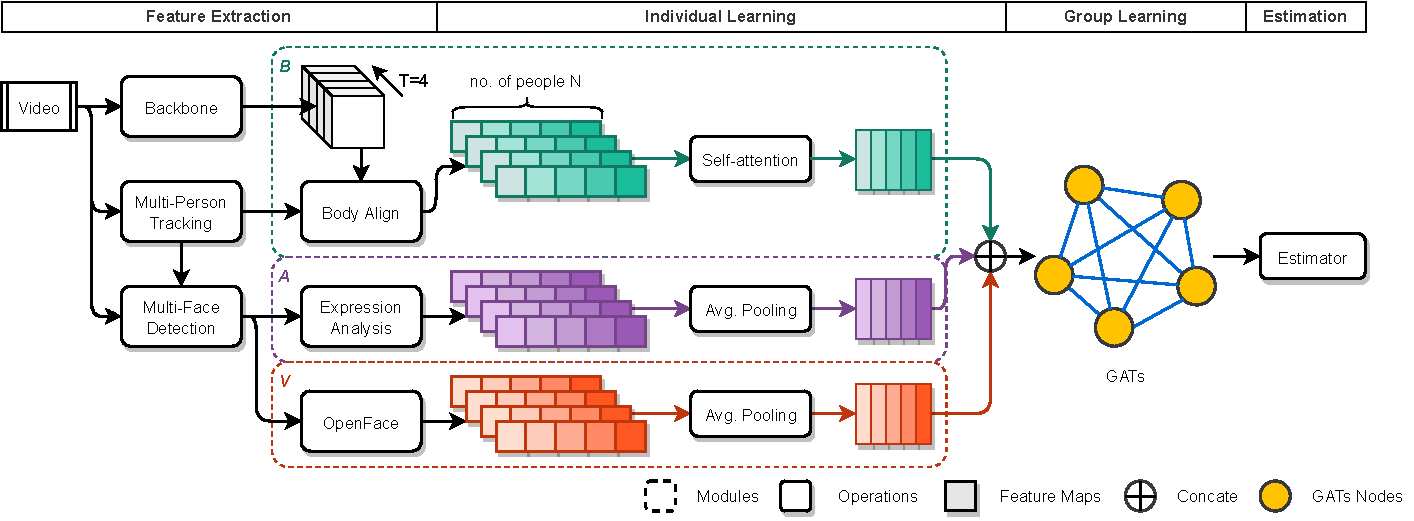
\includegraphics[width=\linewidth]{assets/pipeline_4.drawio}
  \caption{Architecture of the proposed network. We adapt a ResNet-3D model for extracting spatio-temporal features. Multi-person tracking and multi-face detection are used to get the bounding boxes in order to align and slice out corresponding body and face feature maps, which are then pooled for individual learning. \textcolor{red}{Three-branch self-attention mechanism is applied to refine the feature maps, \ie, learning the behavioral ($\mathcal{B}$), affective ($\mathcal{A}$), and visual ($\mathcal{V}$) engagement, respectively. The concatenation of these learned three components is the final representation of an individual.}}
  \label{f:pipeline_4}
\end{figure*}

% ========================= APPROACH ============================
% ========================= APPROACH ============================
\section{Proposed Method}
\label{s:Engagement_Estimation_of_the_Elderly}



%Our problem can be described as follows. The input is raw video recordings of the elderly-robot interaction. Formally, we denote the dataset by $\mathcal{V} = \{V_1, ..., V_m, ..., V_M\}$ where $V_m$ is the video recordings of an interaction session $m$. For each interaction session, normally there is only one old participant $p$. The session consists of $K$ video clips denoted by $V_m = \{v_m^1, ..., v_m^k, ..., v_m^K\}$ where $K$ may vary from session to session. It is assumed that each video clip is associated with a value $y_m^k \in [0, 1]$ representing the elderly's engagement state in this video clip. The value 0 represents the lowest level of engagement and the value 1 represents the highest level of engagement. Our goal is to develop a method to estimate the value of engagement $\hat{y}_m^k$.

Our problem can be described as follows. The input is a raw video clip of the elderly-robot interaction in a wild multiparty environment. This video clip has a duration of about 10 seconds and contains only one elderly as the main participant and possibly a few other participants. It is assumed that within this duration the elderly's engagement state is fixed and corresponds to a value in $[0, 1]$. The value 0 represents the lowest level of engagement and the value 1 represents the highest level of engagement. Our goal is to estimate the value of engagement. In real applications, a human-robot interaction usually contains several interaction sessions and each session can be further divided into a sequence of clips. If we can estimate the value of engagement for each clip, we can obtain the engagement state over the entire interaction sessions.  

In this section we present a machine learning method for estimating the value of engagement of the elderly given a video clip. The method consists of four modules.
%The overview of the method is shown in Fig.~\ref{f:architecture}. 
The first module is feature extraction. We use some the pre-trained network models to obtain spatio-temporal representations of the input videos, from which behavior, affective and visual face features are extracted. The second module is individual learning, which refines individual features by adding a self-attention mechanism. Because the facial features and body movements of older adults are difficult to recognize, we introduce the attention mechanism to enrich individual features. The third module is group learning. We construct a graph network to learn the response from nurses as well as the relationships of participants within the group, which further helps to understand the engagement of the elderly. The last module is engagement estimation, which outputs a value representing the elderly's engagement state. This is done just simply by a fully connected layer. Fig.~\ref{f:pipeline_4} gives the overall architecture of the proposed method. We next elaborate the first three modules in detail.



\subsection{Feature Extraction}
\label{subs:Feature_Extraction}

We use ResNet-3D as the backbone to capture spatio-temporal context of an input video clip. This is motivated by the promising performance of ResNet-3D models~\cite{Hara2018Can} in a wide range of video-related benchmarks~\cite{Chen2021Deep}, we employ the feature representations extracted by this backbone pre-trained on Kinetics 400~\cite{Kay2017Kinetics}. The model details are listed in Table~\ref{t:resnet3d}. We use the output, $X^B_{r4} \in \mathbb{R}^{1024\times4\times14\times14}$, from $res_4$ layer as the spatio-temporal feature maps, representing the behavioral engagement. Here, 1024 is the channel depth; 4 is the temporal dimension; and $14\times14$ is the map size. As depicted in Fig.~\ref{f:pipeline_4}, we extract four feature maps in time positions from this representation.

\begin{table}[htb]
  \centering
  \caption{The structure of our backbone model.}
  \label{t:resnet3d}
  \begin{tabular}{ccc}
  \toprule
  \textbf{Layer name} & \textbf{Architecture} & \textbf{Output size} \\
  \midrule
  conv1 & $5\times7\times7$, stride 2, 2, 2 & $16\times112\times112$ \\
  \midrule
  maxpool1 & $2\times3\times3$, stride 2, 2, 2 & $8\times56\times56$ \\
  \midrule
  res2 & $\left[ \begin{array}{c} 3\times1\times1, 64 \\ 1\times3\times3, 64 \\ 1\times1\times1, 256 \end{array}\right]\times3$ & $8\times56\times56$ \\
  \midrule
  maxpool2 & $2\times1\times1$, stride 2, 1, 1 & $4\times56\times56$ \\
  \midrule
  res3 & $\left[ \begin{array}{c} 3\times1\times1, 128 \\ 1\times3\times3, 128 \\ 1\times1\times1, 512 \end{array}\right]\times4$ & $4\times28\times28$ \\
  \midrule
  res4 & $\left[ \begin{array}{c} 3\times1\times1, 256 \\ 1\times3\times3, 256 \\ 1\times1\times1, 1024 \end{array}\right]\times6$ & $4\times14\times14$ \\
  \bottomrule
  \end{tabular}
\end{table}

Meanwhile, we conduct multi-person tracking on each input video clip. The purpose of this step is threefold: (i) the main interaction participants are identified based on these bounding boxes; (ii) we use these bounding boxes to further focus on the people and eliminate the interference of redundant background information; (iii) the tracked bounding boxes are used as constraints for face tracking as a way to ensure the consistency of face and body information.

To do this, we first perform multi-person tracking (MPT) using ByteTrack~\cite{Zhang2021ByteTrack} to gain the bounding boxes (BBX) of the detected bodies. We use an intuitive approach for the main group member identification, based on the frequency of a person's appearance in temporal axis and the distance from the camera in space axis. Here, we evaluate distance by the size of the BBX. We set the frequency threshold to be 20\% and minimum BBX size as 5000.

Given these, we use RoI Align~\cite{He2017Mask} to project the coordinates on the frames' feature maps and slice out the corresponding features for each individual, after which behavioral feature maps are revised to $X^B \in \mathbb{R}^{N\times1024\times4\times7\times7}$, where $N$ is the number of detected participants. Formally,
\begin{equation}
  X^B = RoI\left(E\left(v_m^k\right), {\rm BBX}\right)
\end{equation}
where video clip $v_m^k$ includes participants of number $N_m^k$. $RoI$ and $E$ are RoI Align and feature extraction operations, respectively. For simplifying the notations, we will eliminate $m$ and $k$ in the following sections.

To extract affective and visual engagement features, we first perform multi-face detection by RetinaFace~\cite{Deng2020RetinaFace}. In order to ensure the consistency of the face and body in the temporal dimension, we keep $T = 4$ in temporal position. The detected $N\times4$ faces are used for later affective and visual feature extraction.

For affective features, we apply a pre-trained emotion recognition model, DMUE~\cite{She2021Dive}, on the cropped and aligned faces. To keep more facial information, we do not use the original 8 emotion classification results, but instead, we remove the final linear projection layer and use the mid-output to represent affective engagement, resulting the affective features $X^A \in \mathbb{R}^{N\times4\times512}$.

Also, we use OpenFace~\cite{Baltrusaitis2018OpenFace} to extract the visual features. Since visual engagement is highly related to head and eyes behavioral, we select head pose and gaze features. Specifically, 6 head pose, 6 gaze directions and 2 gaze angles, 112 2D eye region landmarks, and 168 3D landmarks are extracted here, which together form the visual engagement features $X^V \in \mathbb{R}^{N\times4\times294}$.

%%%%%%%%%%%%%%%%%%%%%%%%%%
\subsection{Individual Learning}
\label{subs:Individual_Learning}

In the behavioral branch of individual learning, we introduce a self-attentive mechanism to further optimize the representation of the behavioral features. We hope that the attention mechanism can explore important information between any two feature positions in spatio-temporal dimensions and then refine the feature representations, \ie, focusing more on the important body regions in the spatial domain and the critical frames in the temporal domain. As demonstrated by ablation studies in Sec.~\ref{s:Experiments_and_Results}, capturing such fine details contributes to the improvement of estimation performance.

In our work, the self-attention mechanism is a non-local operation~\cite{Wang2018NonLocal}, which calculates the response at a given position as a weighted sum of the features at all positions. In particular, the self-attention block receives behavioral feature maps $X^B$ extracted from the previous module as input and outputs optimized representations. The non-local block is shown in Fig.~\ref{f:self-attention}. $X^B$ is fed into three separate convolutions to embed the feature map. The operation $f$ computes the relationship between different locations, which is an item of the non-local operation, along with $g$, a simple linear embedding. Then, a residual connection is applied, followed by an average pooling to down sampling feature maps to the size of $N\times1024$.

\begin{figure}[t]
  \centering
  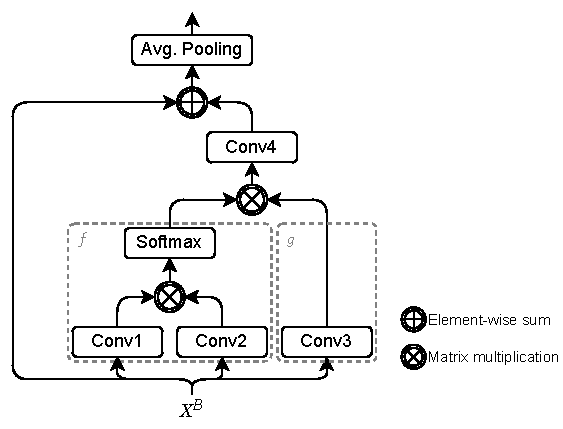
\includegraphics[width=0.9\linewidth]{assets/self-attention.drawio}
  \caption{Self-attention block. The convolutional layers are all with kernel size of $1\times1\times1$, but have different weights.}
  \label{f:self-attention}
\end{figure}

For affective and visual features, because of the relative small feature dimension, we do not apply self-attention mechanism on them. Instead, we simply apply an average pooling (AP), which works on the temporal dimension, to make affective and visual features have appropriate size with the behavioral features.

Finally, we concatenate the three individual's features to derive the refined individual feature map:
\begin{equation}
\label{eq:h}
  \mathbf{H} = \left[\alpha\left(X^B\right), {\rm AP}\left(X^A\right), {\rm AP}\left(X^V\right)\right].
\end{equation}
where $\alpha$ is the attention operation.

Note that in Eq.~\ref{eq:h}, $\mathbf{H}$ is represented in terms of feature types. We reorganize it according to the detected people. Without ambiguity, we still use the notation $\mathbf{H}$, i.e., $\mathbf{H} = \left[h_1, ..., h_N\right]$, where each $h_i$ contains behavioral, affective, and visual features obtained from individual learning, and $\left[\cdot, \cdot\right]$ denotes concatenation. This $\mathbf{H}$ is then used as the input to the next module: group learning.


%%%%%
\subsection{Group Learning}
\label{subs:Group_Learning}

Engagement estimation of the elderly relies on subtle interactions among individuals present in a multiparty HRI scenario. It has been known that estimating engagement solely from the elderly is not very reliable. In fact, in the elderly-nurse-robot interaction scenario, nurses are not just the auxiliaries and participants of the interaction. They are also the people who are in daily contact with the elderly and hence they have the prompt judgment about the expressions of the elderly. These judgments are conveyed in their behaviors. 

Generally in human conversation, each participant plays a specific role: speaker, addressee, or side-partic- ipant who is part of the group of potential speakers but is currently taking on a listening role~\cite{Goffman1981Forms,Clark1996Using}. In a wild dynamic multiparty interaction, we define the main interaction group to be composed of these participants including speaker, addressee and side-participants. The rest, who may be bystanders and overhearers, is called the background.
In the elderly-nurse-robot interaction scenario described above, we hypothesize that \textit{analyzing all participants in the main interaction group and their relationships helps to estimate the engagement of the individual elderly.} 

To represent the main interaction group, we propose to use the graph structure where each node corresponds to a participant and stores his/her feature map, and each edge represents the interaction between the participants of the two nodes. We further build graph neural networks (GNNs)~\cite{Scarselli2008Graph} to learn the graph representation, which is to compute the hidden representation of each node in the graph by attending over its neighbors.  Specifically, we assign an attention weight to each edge and adapt GATs~\cite{Velivckovic2017Graph} to learn the underlying interactions between nodes. 

We construct our graph attention layer (GAL) as follows. GAL takes $\mathbf{H} = \{h_1, ..., h_N\}$ that derived from individual learning and produces a new set of features $\mathbf{H}^{\prime}  = \{h_1^{\prime}, ..., h_N^{\prime}\}$. A shared linear transformation with the weight matrix $W$ is applied to every node. We then perform self-attention $a$ to compute attention coefficients
\begin{equation}
  e_{ij} = a\left(Wh_i,Wh_j\right)
\end{equation}
that indicate the importance of node $j$'s features to node $i$. The model allows every node to attend on other nodes. To make coefficients easily comparable across different nodes, we normalize them across all choices of $j$ using the softmax function:
\begin{equation}
  \alpha_{ij} = {\rm softmax}_j(e_{ij}) = \frac{{\rm exp}(e_{ij})}{\sum_{k \in \mathcal{N}}{\rm exp}(e_{ik})}.
\end{equation}

In our experiments, the attention mechanism $a$ is a single-layer feedforward neural network, parameterized by a weight vector $\mathbf{a}$, and applying the LeakyReLU nonlinearity (with negative input slope $\alpha = 0.2$). Fully expanded out, the coefficients computed by the attention mechanism (illustrated by Fig.~\ref{f:gats}) may then be expressed as
\begin{equation}
  \alpha_{ij} = \frac{{\rm exp}({\rm LeakyReLU}(\mathbf{a}^T[Wh_i,Wh_j]))}{\sum_{k \in \mathcal{N}}{\rm exp}({\rm LeakyReLU}(\mathbf{a}^T[Wh_i,Wh_k]))}.
\end{equation}

\begin{figure}[t]
  \centering
  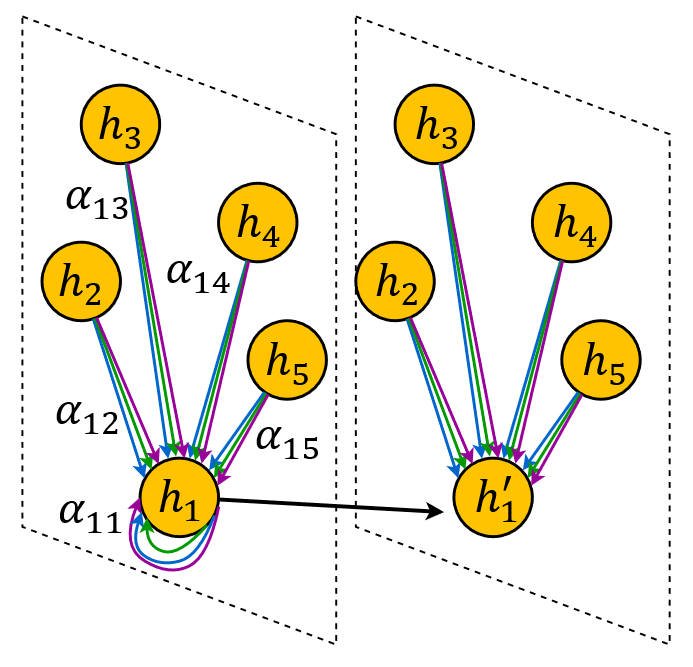
\includegraphics[width=0.5\linewidth]{assets/gats_3}
  \caption{Schematic diagram of GATs by node 1 on its neighborhood. The aggregated features from each head are concatenated to obtain $h_1^{\prime}$. The arrows to node 1 are from multi-head architecture.}
  \label{f:gats}
\end{figure}

The normalized attention coefficients are used to compute a linear combination of the features corresponding to them, as the final features for every node (after potentially applying a nonlinearity, $\sigma$):
\begin{equation}
  h_i^{\prime} = \sigma\left(\sum_{j \in \mathcal{N}} \alpha_{ij}Wh_j\right).
\end{equation}

To stabilize the learning process of self-attention, we employ multi-head structure, where $K$ independent attention mechanisms execute the transformation and then their features are concatenated
\begin{equation}
  h_i^{\prime} = \left[\sigma\left(\sum_{j \in \mathcal{N}} \alpha_{ij}^1W^1h_j\right),...,\sigma\left(\sum_{j \in \mathcal{N}} \alpha_{ij}^KW^Kh_j\right)\right]
\end{equation}
$\alpha_{ij}^k$ is normalized attention coefficients computed by the $k$-th attention mechanism ($a^k$), and $W^k$ is the corresponding input linear transformation's weight matrix. Finally, We use the updated node information to generate the final engagement value $y^{\prime}$ by a FC estimator.



We formulate our task as a regression problem, We replace the final layer and the loss function for training is constructed based on the mean squared error (MSE):
\begin{equation}
  MSE = \frac{1}{N}\sum_{i=1}^N(y_i-\hat{y})^2,
\end{equation}


% ======================== EXPERIMENTS ==========================
\section{Experiments and Results}
\label{s:Experiments_and_Results}
This section reports our experiments, which include dataset labeling, implementation detail, main results, and ablation studies.

\subsection{BHEH Dataset}
\label{subs:BHEH_Dataset}

To the best of our knowledge, there is no publically available labeled dataset for learning elderly-robot interaction, not mentioning in a multiparty scenario. In our experiments, we use BHEH dataset, which was collected in a project that studied the interaction of the elderly with a socially intelligent humanoid robot at Bright Hill Evergreen Home (BHEH), Singapore. 
%NTU Institutional Review Board has approved this study. A detailed consent form was signed before the onset of the procedure, followed by a detailed explanation of the experiment. 
29 participants aged 60 years above participated in the project. They were people with dementia. The BHEH dataset  is a video recording of real elderly-robot interaction. There is no constraint imposed on the participants. The elderly talked to a humanoid robot while the nurses occasionally provided help. Moreover, the dataset is collected in a wild, dynamic, and multiparty environment. In the background, nurses may pass through the scene; some old people may sit near to or far from the interaction group; the interaction participants may leave and join at any time. 
More detailed information of the dataset and the research setting can be found in \cite{Mishra2021Does, Tulsulkar2021Can}.

\begin{figure}[t]
  \centering
  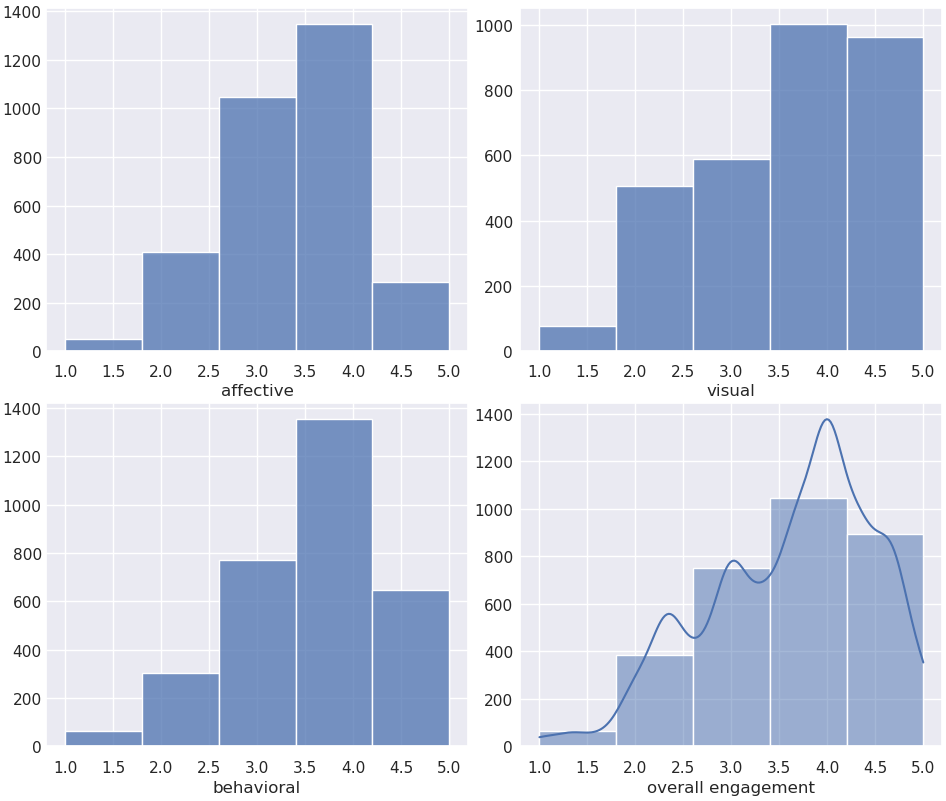
\includegraphics[width=\linewidth]{assets/label_overview}
  \caption{Overview of the engagement annotation. X-axis and y-axis represent engagement value and clip count.}
  \label{f:label_overview}
\end{figure}

We annotate 43 interaction sessions in 4 months with 16 older people attending the experiments. The length of the video is between 3 and 38 minutes (over 560 minutes in total). The participants number for each session is from 2 to 6. 

The label of the data is the engagement score, which is gained based on  EPWDS~\cite{Jones2018Engagement}. By removing two components that are less relevant to our problem, we simplified EPWDS for artificial engagement annotation. The details of the annotation form is shown in Fig.~\ref{f:annotation_form}. Each interaction session is at least annotated by two experts. Fig.~\ref{f:label_overview} illustrates the labelled engagement.  

\begin{figure*}[t]
  \centering
  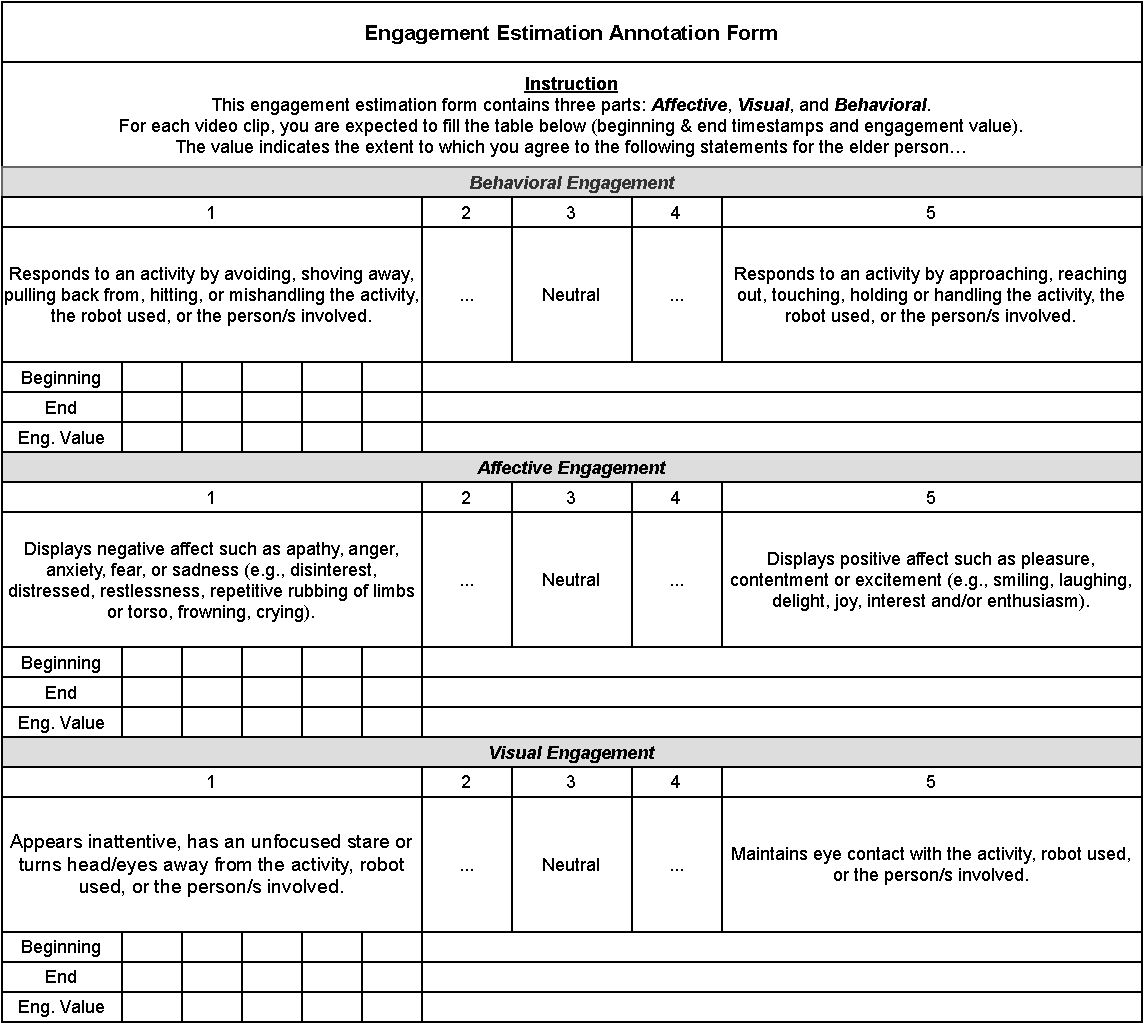
\includegraphics[width=\linewidth]{assets/annotation_form.drawio}
  \caption{Engagement Estimation Annotation Form}
  \label{f:annotation_form}
\end{figure*}




%%%%%%%%%%%%%%%%%%%%%%%%%
\subsection{Implementation Details}
\label{subs:Implementation_Details}

The original video was collected in 15 fps. To extract video features by the pre-trained networks, we sampled the videos by selecting one frame from every 5 frames. As a result, for each video clip that records the interaction for about 10.67 seconds, we get 32 frames that are used as the input to our method. 

We randomly selected 80\% of clips as the training set and the rest was for testing. In our model, we adapted a pretrained ResNet-3D as the backbone, followed by RoI Align with crop size of $7\times7$. We performed the self-attention on individuals' feature map by a spacetime non-local block with embedded Gaussian bottleneck. Individuals' feature maps were fed into a single-layer, 3-head GATs module with hidden size 64, dropout rate 0.5, and $\alpha = 0.2$. We trained our model in two stages. The individual learning module was trained first, and then we fine-tuned the network end-to-end including GATs. Both steps were trained using Adam optimizer in 120 epochs with initial learning rate $10^{-3}$, divided by 10 every 50 epochs. MSE loss is used in the entire training process.

\subsection{Results}
\label{subs:Main_Results}

We compare our proposed method with the state-of-the-art methods in engagement estimation. However, there are no publicly available datasets and benchmarks in this domain. Moreover, the scenarios of HRI involved in the state-of-the-art are very different, and thus the results may appear different on different datasets.
All these make it very difficult to have a fair comparison. We apply the prior art methods to our dataset which may be a compromise approach. It should be pointed out that the prior art methods we compare with do not publish their codes, so we did our best to re-implement them.

\begin{table}[htb]
  \centering
  \caption{Engagement Estimation of the Elderly.}
  \label{t:main_results}
  \begin{tabular}{cccc}
  \toprule
  \textbf{} & \textbf{MSE} & \textbf{MAE} \\
  \midrule
  2D CNNs~\cite{Anagnostopoulou2021Engagement} & 0.1104 & 0.4123 \\
  Inception V2~\cite{Saleh2021Improving} & 0.0235 & 0.1401 \\
  LSTM~\cite{Steinert2020Engagement} & 0.1471 & 0.3170 \\
  % LSTM~\cite{Sumer2021Multimodal} &  & \\
  \midrule
  \textbf{Ours}& \textbf{0.0142} & \textbf{0.0773} \\ % & \textbf{0.0094} 
  \bottomrule
  \end{tabular}
\end{table}

\begin{figure}[t]
  \centering
  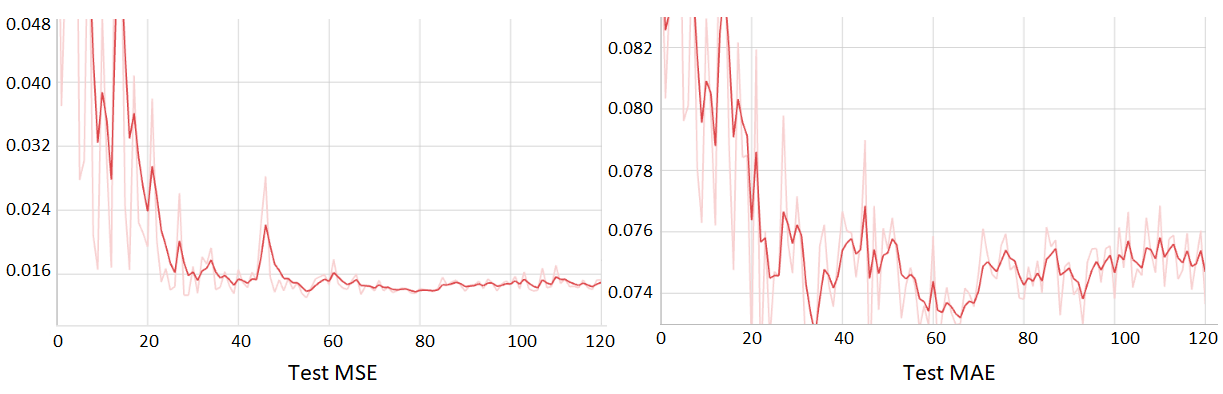
\includegraphics[width=\linewidth]{assets/loss}
  \caption{Losses of MSE and MAE on testing set.}
  \label{f:loss}
\end{figure}

For 2D CNNs~\cite{Anagnostopoulou2021Engagement}, as our inputs are just RGB videos without depth information, we adopt its 2D body pose as features and use AlexNet as the comparison model, which achieves most top performance in its paper. Inception V2~\cite{Saleh2021Improving} has the same input format as ours, so the implementation just follows its light-inception model architecture. In \cite{Steinert2020Engagement}, LSTM is used to classify engagement based on extracted OpenFace and VGG features. To make fair comparisons, we use the same frame length. For evaluation, we use two metrics: MSE and mean absolute error (MAE):
\begin{equation}
  MAE = \frac{1}{N}\sum_{i=1}^N|y_i-\hat{y}|.
\end{equation}

The results are reported in Table~\ref{t:main_results}. The testing losses are shown in Fig.~\ref{f:loss}. The performance of our model (MSE=0.0142) outperforms the prior art. Some outputs are visualized in Fig.~\ref{f:visualization}. It can be seen that our method achieves good results even under challenging conditions. For better understanding, we demonstrate three estimation examples where the first column is the center frame of the example clip, followed by group detection, behavioral representation from body align, affective and visual representation, and estimation results. In example 1, 5 people's bodies are detected and used for later feature extraction, but the leftmost person is not desired. This is a false example of the main group detection. In contrast, examples 2 and 3 detect all the participants successfully. In terms of affective and visual engagement representation, some inconsistency and instability are involved due to the masks and senescent faces, \eg, the elderly in example 1 cannot make meaningful expressions, and the visual features in example 3 are also missed. This might be the reason of the dissatisfied results for those methods only involving facial information. In addition, both elderly from example 1 and 3 are not good at body language, so the information from side participants helps in the estimation, \eg, the body representation captures the raised hand of the nurse.

\begin{figure*}[t]
  \centering
  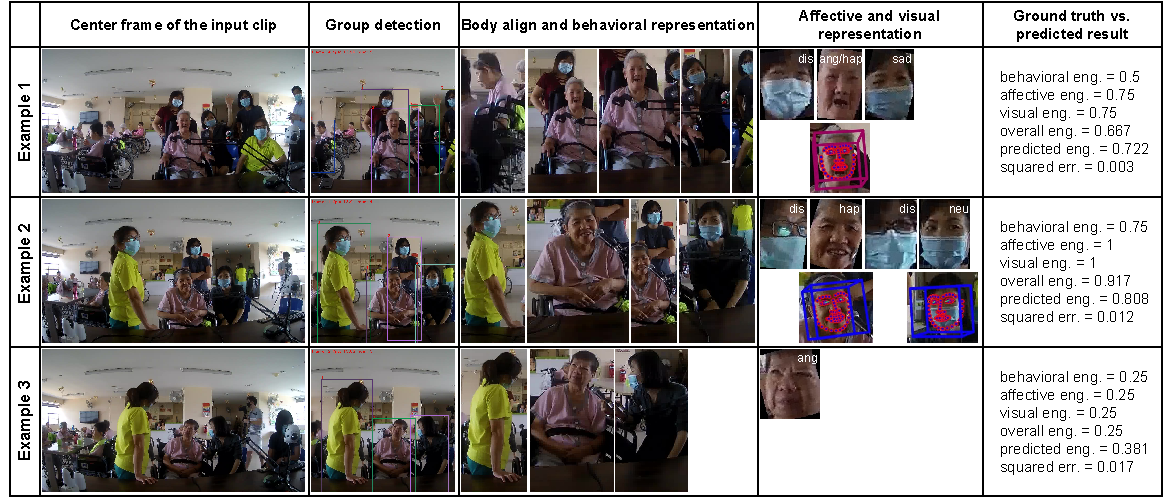
\includegraphics[width=\linewidth]{assets/visualization.drawio}
  \caption{Visualization of the engagement estimation results.}
  \label{f:visualization}
\end{figure*}

\subsection{Ablation Studies}
\label{subs:Ablation_Studies}

We run a number of ablations to analyze our method. The results are given in Table~\ref{t:ablations}. $\mathcal{B}$, $\mathcal{A}$, and $\mathcal{V}$ are the results of using a single engagement element of behavioral, affective, and visual. It can be seen that the results underperform the proposed multi-element method. The self-attention module also helps improve the performance by 0.0425 in MSE and 0.1357 in MAE. By employing the GATs in our group learning module, the results have 0.0171 increase in MSE, which means that the signals from side-participants contribute to the estimation in our multiparty elderly-robot interaction.

\begin{table}[t]
  \centering
  \caption{Ablation results.}
  \label{t:ablations}
  \begin{tabular}{ccc}
  \toprule
  \textbf{} & \textbf{MSE} & \textbf{MAE} \\
  \midrule
  $\mathcal{B}$ & 0.0451 ($\downarrow$0.0309) & 0.1750 ($\downarrow$0.0977) \\
  $\mathcal{A}$ & 0.1235 ($\downarrow$0.1093) & 0.3690 ($\downarrow$0.2917) \\
  $\mathcal{V}$ & 0.1567 ($\downarrow$0.1425) & 0.4184 ($\downarrow$0.3411) \\
  % $\mathcal{B,A}$ &  & \\
  % $\mathcal{B,V}$ &  & \\
  % $\mathcal{A,V}$ &  & \\
  w/o self-attention & 0.0567 ($\downarrow$0.0425) & 0.2130 ($\downarrow$0.1357) \\
  w/o GATs & 0.0313 ($\downarrow$0.0171) & 0.1091 ($\downarrow$0.0318) \\
  \bottomrule
  \end{tabular}
\end{table}

% ======================== CONCLUSIONS ==========================
\section{Conclusions}
\label{s:Conclusions}

In this paper, we use real-world videos to estimate the engagement of old people in a multiparty human-robot interaction scenario. We perform analysis and feature extraction on three engagement components. The proposed deep learning architecture explores both individual and group information. Our experiments show that the proposed framework achieves good performance in the engagement estimation task.

% ======================== APPENDICES ===========================
%\section{Appendix}
%\label{ap:annotation_form}

% ======================== REFERENCES ===========================
\bibliographystyle{spmpsci}
\bibliography{CGI22}

\end{document}
